\lhead[\thepage]{CAPÍTULO \thechapter. ESTADO DE LA CUESTIÓN}
\chead[]{}
\rhead[Patrones de programación paralelos de alto nivel en arquitecturas de memoria distribuida\leftmark]{\thepage}
\renewcommand{\headrulewidth}{0.5pt}

\lfoot[]{}
\cfoot[]{}
\rfoot[]{}
\renewcommand{\footrulewidth}{0pt}

%% This is an example first chapter.  You should put chapter/appendix that you
%% write into a separate file, and add a line \include{yourfilename} to
%% main.tex, where `yourfilename.tex' is the name of the chapter/appendix file.
%% You can process specific files by typing their names in at the 
%% \files=
%% prompt when you run the file main.tex through LaTeX.
\chapter{Estado de la cuestión}
\label{ch:estado_de_la_cuestion}
\markboth{}{ESTADO DE LA CUESTIÓN}

Este capítulo presenta el estado de la cuestión, la última y más avanzada etapa de las tecnologías relacionadas con nuestra solución. Primero, discutimos los principales paradigmas de programación paralela (Sección \ref{sec:paradigmas_programacion_paralela}). Después, presentamos los principales frameworks de programación paralela disponibles (Sección \ref{sec:frameworks_programacion_paralelos}). Finalmente, se exponen los frameworks basados en patrones paralelos (Sección \ref{sec:frameworks_basados_patrones}). 

\section{Paradigmas de programación paralela}
\label{sec:paradigmas_programacion_paralela}

En los últimos 50 años, se han realizado grandes avances en el rendimiento y la capacidad de un sistema informático. Estos avances han sido posibles gracias a la ayuda de la tecnología \acrshort{vlsi}. La tecnología \acrshort{vlsi} permite que una gran cantidad de componentes se alojen en un solo chip y aumenten las velocidades de reloj. Por lo tanto, se pueden realizar más operaciones a la vez, en paralelo.

El procesamiento en paralelo también está asociado con la ubicación de datos y la comunicación de datos. Las arquiteturas paralelelas son el método de organizar todos los recursos para maximizar el rendimiento y la programabilidad dentro de los límites dados por la tecnología y el coste en cualquier instancia de tiempo. Estas arquitecturas agregan una nueva dimensión en el desarrollo del sistema informático al usar cada vez más procesadores. En principio, el rendimiento logrado al utilizar una gran cantidad de procesadores es más alto que el rendimiento de un solo procesador en un momento determinado. Con el avance de la capacidad del hardware, también aumentó la demanda de prestaciones, siendo necesario el desarrollo de la arquitectura de la computadora. 

Antes de la era de los microprocesadores, se obtenía un sistema informático de alto rendimiento mediante tecnología de circuitos específicos y organización de máquinas, lo que resultaba muy costoso. Actualmente, el sistema informático de alto rendimiento se obtiene mediante el uso de múltiples procesadores, y las aplicaciones más importantes y exigentes se escriben como programas paralelos. Por lo tanto, para un mayor rendimiento, se necesitan desarrollar arquitecturas paralelas y aplicaciones paralelas.

Las máquinas paralelas se han desarrollado con varias arquitecturas distintas. La arquitectura paralela mejora los conceptos convencionales de la arquitectura de la computadora con la arquitectura de comunicación. La arquitectura de la computadora define las abstracciones críticas (como el límite del sistema del usuario y el límite del software/hardware) y la estructura de la organización, mientras que la arquitectura de comunicación define las operaciones básicas de comunicación y sincronización. También aborda la estructura organizacional. El modelo de programación es la capa superior. Las aplicaciones están escritas en el modelo de programación. Los modelos de programación paralela \cite{sharedVsMpi}, \cite{nitzberg1991distributed} incluyen memoria compartida, paso de mensajes y paralelismo de datos, los cuales son descritos a continuación.

\subsection{Memoria compartida}
\label{sec:memoria_compartida}
Los multiprocesadores de memoria compartida son una de las clases más importantes de máquinas paralelas. Proporciona un mejor rendimiento en cargas de trabajo de multiprogramación y admite programas paralelos. En este caso, todos los sistemas informáticos permiten que un procesador y un conjunto de controladores de E/S accedan a una colección de módulos de memoria mediante alguna interconexión de hardware. La capacidad de la memoria aumenta al agregar módulos de memoria y la capacidad de E/S aumenta al agregar dispositivos al controlador de E/S o al agregar un controlador de E/S adicional. La capacidad de procesamiento se puede aumentar esperando a que esté disponible un procesador más rápido o agregando más procesadores.

Todos los recursos están organizados alrededor de un bus de memoria central. A través del mecanismo de acceso al bus, cualquier procesador puede acceder a cualquier dirección física en el sistema. Como todos los procesadores son equidistantes de todas las ubicaciones de memoria, el tiempo de acceso o la latencia de todos los procesadores es el mismo en una ubicación de memoria. Esto se llama multiprocesador simétrico \cite{bertogna2007response}.

Los dos modelos de multiprocesadores de memoria compartida más relevantes son:

\begin{itemize}
    \item \textbf{\textit{Acceso a memoria uniforme (\acrshort{uma})}}: En este modelo, todos los procesadores comparten la memoria física de manera uniforme \cite{rogers2013amd}. Todos los procesadores tienen igual tiempo de acceso a todas las palabras de memoria. Cada procesador puede tener una memoria caché privada. La misma regla se sigue para los dispositivos periféricos. Cuando todos los procesadores tienen el mismo acceso a todos los dispositivos periféricos, el sistema se denomina multiprocesador simétrico. Cuando solo uno o unos pocos procesadores pueden acceder a los dispositivos periféricos, el sistema se denomina multiprocesador asimétrico.
    
\vspace{0.35cm}
\begin{figure}[h]
 	\centering
 	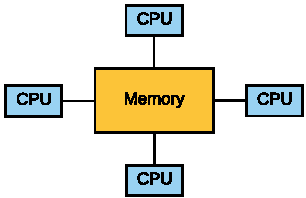
\includegraphics[width=11.5cm]{figures/UMA}
 	\caption{Esquema de arquitectura \acrshort{uma}.}
 	\label{fig:chap2:UMA}
\end{figure}
\vspace{0.35cm}
    
    \item \textbf{\textit{Acceso a memoria no uniforme (\acrshort{numa})}}: En el modelo de multiprocesador \acrshort{numa} \cite{numa}, el tiempo de acceso varía según la ubicación de la palabra de memoria. Aquí, la memoria compartida se distribuye físicamente entre todos los procesadores, llamadas memorias locales. La colección de todas las memorias locales forma un espacio de direcciones global al que pueden acceder todos los procesadores.

\vspace{0.35cm}
\begin{figure}[h]
 	\centering
 	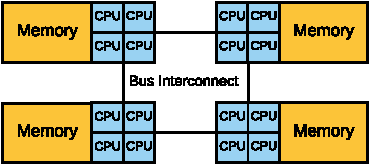
\includegraphics[width=11.5cm]{figures/NUMA}
 	\caption{Esquema de arquitectura \acrshort{numa}.}
 	\label{fig:chap2:NUMA}
\end{figure} 
\vspace{0.35cm}
    
\end{itemize}

El modelo de programación de memoria compartida depende de los procesadores multi-core de memoria compartida. Estos modelos de programación se comunican al compartir los datos en el espacio de direcciones global. Suponen que todos los procesos paralelos pueden acceder a todo el conjunto de memoria. Por ello, es importante lograr consistencia en los datos \cite{gharachorloo1990memory}, ya que diferentes procesadores pueden comunicarse compartiendo el mismo el mismo dato. Para resolver este problema, se utilizan los protocolos de coherencia de caché \cite{cacheprotocol}. La comunicación entre procesos paralelos debe realizarse haciendo uso de diferentes primitivas de sincronización de procesos como los bloqueos o la memoria transaccional \cite{hammond2004transactional}. Estos modelos de programación, proporcionan una serie de ventajas y desventajas que son expuestas a continuación:

\vspace{0.35cm}
\begin{table}[htbp]
\ra{1}
\centering
%\resizebox{\textwidth}{%
\resizebox{\textwidth}{!}{
\begin{tabular}{@{}l@{}}
\toprule
\textbf{Ventajas}\\ 
\midrule
\cmark Facilitan el desarrollo sencillo de la aplicación en comparación con los sistemas basados en memoria distribuida. \\
\cmark Evitan la multiplicidad de los datos, adoptando esa responsabilidad el modelo y quitándosela al programador. \\
\cmark Ofrecen un mejor rendimiento que los modelos de programación paralela basados en memoria distribuida. \\ 
\midrule
\textbf{Desventajas}\\
\midrule
\xmark Los requisitos de hardware para estos modelos son muy altos y complejos, de forma que incrementa los costes. \\
\xmark En ocasiones se encuentran carreras de datos y \emph{deadlocks} durante la ejecución de las aplicaciones.\\
\bottomrule
\end{tabular}
}
\caption{Ventajas y desventajas de las arquitecturas basadas en memoria compartida.}
\label{tab:shared_memory}
\end{table}
\vspace{0.35cm}

En la actualidad, existen diferentes modelos de programación paralelos basados en memoria compartida. El modelo de hilos \cite{kleiman1996programming} está basado en la biblioteca de hilos que proporciona rutinas de bajo nivel para la paralelización de las aplicaciones. Estos modelos utilizan bloqueos de exclusión mutua y variables condicionales para establecer las comunicaciones y sincronizaciones entre los diferentes hilos. Las ventajas y desventajas que proporciona este modelo son las siguientes:

\vspace{0.35cm}
\begin{table}[htbp]
\ra{1}
\centering
%\resizebox{\textwidth}{%
\resizebox{\textwidth}{!}{
\begin{tabular}{@{}l@{}}
\toprule
\textbf{Ventajas}\\ 
\midrule
\cmark Es el más adecuado para aplicaciones basadas en la multiplicidad de datos. \\
\cmark Proporciona una alta flexibilidad al programador. \\
\cmark Las bibliotecas de hilos son las más utilizadas, por lo que resulta muy fácil encontrar herramientas para este tipo de desarrollo. \\ 
\cmark El rendimiento de la aplicación puede ser mejorado mediante el uso de esperas condicionales y esperas activas. \\
\cmark Resulta fácil desarrollar rutinas paralelas para modelos de threads. \\
\midrule
\textbf{Desventajas}\\
\midrule
\xmark Resulta complicado escribir aplicaciones que utilicen modelos de threads, ya que establecer una comunicación o sincronización\\
implica una sobrecarga de código que es difícil de gestionar y, por lo tanto, tiene tendencia a causar más errores. \\
\xmark El programador debe ser más cuidadoso al usar datos globales, debido a que esto conduce a carreras de datos, interbloqueos\\
y uso compartido falso.\\
\xmark Los modelos de hilos tienen un bajo nivel de abstracción, que resulta necesario para un mejor modelo de programación. \\
\bottomrule
\end{tabular}
}
\caption{Ventajas y desventajas del modelo de programación basado en threads.}
\label{tab:threading_model}
\end{table}
\vspace{0.35cm}

Otro de estos modelos, es el modelo basado en directivas \cite{lee2012early}. Este modelo utiliza las directivas de compilación de alto nivel para paralelizar las aplicaciones, siendo una extensión de los modelos basados en hilos. Los modelos basados en directivas se ocupan de las características de bajo nivel como la partición, la gestión de los hilos trabajadores, la sincronización y la comunicación entre los hilos. Las ventajas y desventajas que proporciona este modelo son las siguiente:

\vspace{0.35cm}
\begin{table}[htbp]
\ra{1}
\centering
%\resizebox{\textwidth}{%
\resizebox{\textwidth}{!}{
\begin{tabular}{@{}l@{}}
\toprule
\textbf{Ventajas}\\ 
\midrule
\cmark Estos modelos surgieron como un estándar.\\
\cmark Es fácil escribir aplicaciones paralelas haciendo uso de ellos. \\
\cmark Se incurre en menos gastos generales de código y es fácil gestionar el código desarrollado mediante directivas. \\ 
\cmark Este modelo se encuentra en un bajo nivel de abstracción. \\ 
\cmark El programador no necesita considerar problemas como condiciones de carrera e interbloqueos. \\
\midrule
\textbf{Desventajas}\\
\midrule
\xmark Estos modelos son menos utilizados. \\
\xmark Proporciona una baja flexibilidad al programador.\\
\xmark El apoyo de las herramientas al desarrollo es bastante bajo. \\
\bottomrule
\end{tabular}
}
\caption{Ventajas y desventajas del modelo de programación basado en directivas.}
\label{tab:directives_model}
\end{table}
\vspace{0.35cm}

Por último, el modelo de tareas está basado en el concepto de especificar tareas \cite{bal1998approaches} en lugar de hilos como lo hacen otros modelos. Esto se debe a que las tareas son de corto alcance y más ligeras que los hilos. En general, las tareas son 18 veces más rápidas que los hilos en las implementaciones de UNIX y 100 veces más rápidas que los hilos en las implementaciones basadas en Windows \cite{inteltbb2008}, \cite{reinders2007intel}. Una diferencia entre tareas e hilos es que las tareas siempre se implementan en el espacio de usuario \cite{multicorestate}. Además, las tareas son paralelas pero no concurrentes, por lo que no tienen prioridad y pueden ejecutarse de forma secuencial. Las ventajas y desventajas que proporcionan estos modelos son las siguientes:

\vspace{0.35cm}
\begin{table}[htbp]
\ra{1}
\centering
%\resizebox{\textwidth}{%
\resizebox{\textwidth}{!}{
\begin{tabular}{@{}l@{}}
\toprule
\textbf{Ventajas}\\ 
\midrule
\cmark Las tareas disminuyen la sobrecarga asociada con las comunicaciones tal como se observa en otros modelos. \\
\cmark Facilita el desarrollo de las aplicaciones paralelas. \\
\cmark Existe una gran variedad de herramientas relacionadas con los modelos basados en tareas, facilitando la depuración de errores. \\ 
\midrule
\textbf{Desventajas}\\
\midrule
\xmark Estos modelos no figuran como estándar. \\
\xmark Tienen una curva de aprendizaje grande.\\
\xmark La flexibilidad que proporcionan estos modelos es baja.\\
\bottomrule
\end{tabular}
}
\caption{Ventajas y desventajas del modelo de programación basado en tareas.}
\label{tab:tasking_model}
\end{table}
\vspace{0.35cm}

\subsection{Memoria distribuida}
\label{sec:memoria_distribuida}
La arquitectura de memoria distribuida \cite{tanenbaum2007distributed} también es una clase importante de máquinas paralelas. Proporciona comunicación entre procesadores como operaciones explícitas de E/S. En este caso, la comunicación se combina en el nivel de E/S, en lugar del sistema de memoria.

En esta arquitectura, la comunicación del usuario se ejecuta mediante el uso de llamadas al sistema operativo o a la biblioteca que realizan muchas acciones de nivel inferior, que incluyen la operación de comunicación real. Como resultado, hay una distancia entre el modelo de programación y las operaciones de comunicación en el nivel de hardware físico.

\vspace{0.35cm}
\begin{figure}[h]
 	\centering
 	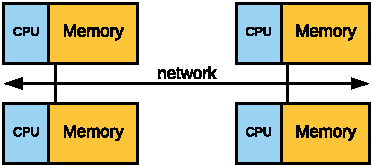
\includegraphics[width=11.5cm]{figures/distributed_memory}
 	\caption{Esquema de arquitectura de memoria distribuida.}
 	\label{fig:chap2:distributed_memory}
\end{figure}  
\vspace{0.35cm}

\emph{Enviar} y \emph{Recibir} son las operaciones de comunicación de nivel de usuario más comunes en este sistema. Enviar especifica un búfer de datos local (que se va a transmitir) y un procesador receptor remoto. Recibir especifica un proceso de envío y un búfer de datos local en el que se colocarán los datos transmitidos. En la operación de envío, se adjunta un identificador o una etiqueta al mensaje y la operación de recepción especifica la regla de coincidencia, como una etiqueta específica de un procesador específico o cualquier etiqueta de cualquier procesador.

La combinación de un envío y una recepción coincidente completa una copia de memoria a memoria. Cada extremo especifica su dirección de datos local y un evento de sincronización por pares.

El modelo más conocido en este tipo de arquitecturas es la arquitectura de memoria solo caché (COMA) \cite{hagersten1999multiprocessing}. El modelo COMA es un caso especial del modelo NUMA. Aquí, todas las memorias principales distribuidas se convierten en memorias de caché. Un sistema de memoria distribuida consta de varias computadoras, conocidas como nodos, interconectadas por la red que pasa mensajes. Cada nodo actúa como una computadora autónoma que tiene un procesador, una memoria local y, a veces, dispositivos de E/S. En este caso, todas las memorias locales son privadas y solo son accesibles para los procesadores locales. Esta es la razón por la cual las máquinas tradicionales se llaman máquinas sin acceso a memoria remota (NORMA).

Este tipo de modelos de programación paralela a menudo se conocen como modelos de paso de mensajes, que permiten la comunicación entre nodos mediante el uso de las rutinas de comunicación de envío/recepción. Los modelos de paso de mensajes evitan las comunicaciones entre procesadores basadas en datos compartidos/globales \cite{multicorestate}. Normalmente, este modelo se utiliza para programar aplicaciones para clusters, donde cada nodo en la arquitectura obtiene su propia instancia de datos e instrucciones. Las ventajas y desventajas de los modelos de programación basados en memoria distribuida son:

\vspace{0.35cm}
\begin{table}[htbp]
\ra{1}
\centering
%\resizebox{\textwidth}{%
\resizebox{\textwidth}{!}{
\begin{tabular}{@{}l@{}}
\toprule
\textbf{Ventajas}\\ 
\midrule
\cmark El requisito de hardware para estos modelos es bajo, menos complejo y tiene un coste pequeño. \\
\cmark Evitan las condiciones de carrera y, como consecuencia, el programador queda liberado de usar los bloqueos.\\
\midrule
\textbf{Desventajas}\\
\midrule
\xmark Encuentran interbloqueos durante el proceso de comunicaciones. \\
\xmark Su desarrollo es difícil y lleva más tiempo.\\
\xmark El desarrollador es responsable de establecer la comunicación entre los nodos.\\
\xmark Están menos orientados al rendimiento y tienen un alto coste de comunicación. \\
\bottomrule
\end{tabular}
}
\caption{Ventajas y desventajas de las arquitecturas basadas en memoria distribuida.}
\label{tab:distributed_memory}
\end{table}
\vspace{0.35cm}

\subsection{Esquemas híbridos}
\label{sec:esquemas_hibridos}

En la actualidad y con motivo de la cada vez mayor necesidad de aumentar el rendimiento de las computadoras, las computadoras más grandes y rápidas en el mundo emplean arquitecturas de memoria compartida y distribuida \cite{rekimoto1999augmented}. Estas máquinas se basan en la unión de los conceptos descritos en las secciones anteriores. El componente de memoria compartida puede ser una máquina de memoria compartida y/o unidades de procesamiento de gráficos (GPU). El componente de memoria distribuida es la conexión en red de varias máquinas de memoria compartida/GPU, que solo conocen su propia memoria, es decir, no conocen la memoria de otra máquina. Por lo tanto, se requieren comunicaciones de red para mover datos de una máquina a otra. Entre las ventajas y desventajas que presentan estos sistemas: 

\vspace{0.35cm}
\begin{table}[htbp]
\ra{1}
\centering
%\resizebox{\textwidth}{%
\resizebox{\textwidth}{!}{
\begin{tabular}{@{}l@{}}
\toprule
\textbf{Ventajas}\\ 
\midrule
\cmark Tiene todas las ventajas propias tanto de un sistema de memoria compartida como de un sistema de memoria distribuida. \\
\cmark El aumento de la escalabilidad es una característica muy importante de estos sistemas.\\
\midrule
\textbf{Desventajas}\\
\midrule
\xmark El aumento de la complejidad del programador es una desventaja muy importante. \\
\bottomrule
\end{tabular}
}
\caption{Ventajas y desventajas de las arquitecturas basadas en esquemas híbridos.}
\label{tab:hybrid_schemas}
\end{table}
\vspace{0.35cm}

\vspace{0.35cm}
\begin{figure}[htbp]
 	\begin{subfigure}{0.5\textwidth}
 	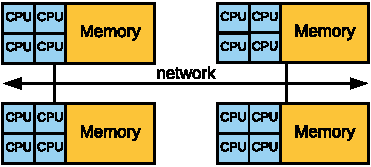
\includegraphics[width=\linewidth]{figures/hybrid_distributed_shared_memory}
 	\caption{Arquitectura de esquemas híbridos sin \acrshort{gpu}.}
 	\label{fig:chap2:hybrid_schemas_1}
 	\end{subfigure}
 	\hspace*{\fill} % separation between the subfigures
 	\begin{subfigure}{0.5\textwidth}
 	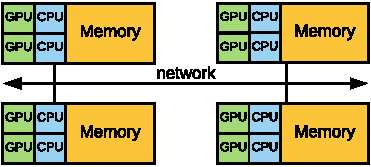
\includegraphics[width=\linewidth]{figures/hybrid_distributed_shared_memory_2}
 	\caption{Arquitectura de esquemas híbridos con \acrshort{gpu}.}
 	\label{fig:chap2:hybrid_schemas_2}
 	\end{subfigure}
 	\caption{Arquitectura esquemas híbridos.}
 	\label{fig:chap2:hybrid_schemas}
\end{figure}  
\vspace{0.35cm}

Las tendencias actuales parecen indicar que este tipo de arquitectura de memoria continuará prevaleciendo e irá en aumento en los próximos años, puesto que gracias a la flexibilidad y escalabilidad que proporciona, permite modificar el sistema con relativa facilidad. A medida que los desarrolladores continúan buscando rendimiento, se les alienta a explorar técnicas de programación híbrida \cite{rabenseifner2009hybrid}, que ofrecen la oportunidad de mejorar el consumo de recursos, especialmente la memoria.

\section{Frameworks de programación paralelos}
\label{sec:frameworks_programacion_paralelos}

Para poder explotar correctamente el funcionamiento de la computadora, los programadores hacen uso de interfaces de programación. Las interfaces de programación suponen que las órdenes de programa no tienen que mantenerse en absoluto entre las operaciones de sincronización. Se garantiza que todas las operaciones de sincronización estén explícitamente etiquetadas o identificadas como tales. La biblioteca de tiempo de ejecución o el compilador traduce estas operaciones de sincronización en las operaciones de preservación de orden adecuadas requeridas por la especificación del sistema.

Por lo tanto, el sistema asegura ejecuciones secuenciales consistentes aunque puede reordenar las operaciones entre las operaciones de sincronización de cualquier forma que desee sin interrumpir las dependencias a una ubicación dentro de un proceso. Esto le permite al compilador suficiente flexibilidad entre los puntos de sincronización para los reordenamientos que desea, y también le otorga al procesador realizar tantos reordenamientos como lo permita su modelo de memoria. En la interfaz del programador, el modelo de coherencia debe ser al menos tan débil como el de la interfaz de hardware, pero no tiene que ser el mismo. A continuación, se exponen los frameworks de programación paralela más relevantes para cada una de las tres arquitecturas descritas en la sección anterior.

\subsection{Memoria compartida}
\label{sec:frameworks_memoria_compartida}

En las arquitecturas multiprocesador de memoria compartida, los hilos se pueden usar para implementar el paralelismo. Históricamente, los proveedores de hardware han implementado sus propias versiones propietarias de hilos, lo que hace que la portabilidad sea una preocupación para los desarrolladores de software. Para los sistemas UNIX, el estándar IEEE POSIX 1003.1c ha especificado una interfaz de programación de hilos de lenguaje C estandarizada. Las implementaciones que se adhieren a este estándar se denominan POSIX threads o Pthreads. Pthreads \cite{nichols1996pthreads} es un modelo de ejecución que existe independientemente del lenguaje, así como un modelo de ejecución paralelo. Permite que un programa controle múltiples flujos de trabajo diferentes superpuestos en el tiempo. Cada flujo de trabajo recibe el nombre de hilo o thread y la creación y el control de estos flujos se realiza mediante llamadas a la \acrshort{api} de subprocesos POSIX. Las implementaciones de la \acrshort{api} están disponibles en muchos sistemas operativos conformes a POSIX tipo Unix, como FreeBSD , NetBSD , OpenBSD , Linux , Mac OS X , Android y Solaris , generalmente empaquetados como biblioteca libpthread . También existen implementaciones de DR-DOS y Microsoft Windows: dentro del subsistema SFU/SUA que proporciona una implementación nativa de varias \acrshort{api} POSIX, y también dentro de paquetes de terceros como pthreads-w32, que implementa Pthreads sobre la \acrshort{api} de Windows existente.

 \acrshort{openmp} \cite{dagum1998openmp}, es un \acrshort{api} para arquitecturas de memoria compartida que proporciona una capacidad multiproceso. Un bucle se puede paralelizar fácilmente invocando llamadas de subrutina desde librerías de hilos \acrshort{openmp} e insertando las directivas del compilador  \acrshort{openmp}. De esta forma, los hilos pueden obtener nuevas tareas y las iteraciones de bucle no procesadas directamente desde la memoria compartida local. \acrshort{openmp} es una especificación abierta para el paralelismo de memoria compartida. La idea básica detrás de \acrshort{openmp} es la ejecución paralela de datos compartidos. Consiste en un conjunto de directivas de compilación, rutinas de biblioteca de tiempo de ejecución y variables de entorno que amplían los programas en los lenguajes de programación FORTRAN, C y C ++. \acrshort{openmp} es portable en la arquitectura de memoria compartida. La unidad de trabajadores en \acrshort{openmp} son los hilos. Cada hilo puede acceder a una variable en memoria caché o memoria \acrshort{ram}. \acrshort{openmp} incluye suporte para las plataformas UNIX y Microsoft Windows. 

Cilk \cite{robison2012cilk}, Cilk ++ y Cilk Plus \cite{blumofe1995cilk} son lenguajes de programación de propósito general diseñados para computación paralela multiproceso . Están basados en los lenguajes de programación C y C++ , que se extienden con construcciones para expresar bucles paralelos y la expresión fork-join. Originalmente desarrollado en la década de 1990 en el Instituto de Tecnología de Massachusetts (\acrshort{mit}), Cilk fue posteriormente comercializado como Cilk++, aumentando su compatibilidad con el código C y C++ tras su compra por parte de Intel. El resultado de este aumento de compatibilidad dió lugar a su nuevo nombre, Cilk Plus.

Entre las abstracciones de hilos más recientes se incluyen Intel Threading Building Blocks (Intel \acrshort{tbb})\cite{inteltbb2008}. Aunque \acrshort{openmp} funciona tanto con C/C ++ como con Fortran, Intel \acrshort{tbb} se basa en plantillas C ++, un modelo de programación genérico, por lo que está limitado a C ++. Debido a que Intel \acrshort{tbb} contiene un amplio conjunto de características, a la vez que proporciona una abstracción clara que es fácil de seguir, se ha vuelto bastante popular entre los programadores de C ++.

El paralelismo anidado es natural tanto para Cilk Plus como para Intel \acrshort{tbb}, en comparación con  \acrshort{openmp}, donde el desarrollador debe identificar y declarar el paralelismo anidado. Esto hace que Intel \acrshort{tbb} y Cilk Plus sean ideales para incluir en las bibliotecas.

\subsection{Memoria distribuida}
\label{sec:frameworks_memoria_distribuida}

Muchas aplicaciones buscaban una mayor potencia de cálculo de la que estaba disponible en un solo sistema multiprocesador. Esto condujo a la conexión de varios sistemas para formar grupos de computadoras para trabajar juntas y resolver una sola carga de trabajo computacional. Estos sistemas vincularon frecuentemente los sistemas junto con un frabricante propietario, con cada plataforma en el clúster que tiene su propia área de memoria privada dentro del clúster. El programa tenía que definir explícitamente los datos que se compartirían con otra plataforma y entregarlos a la otra plataforma en el clúster.

Con el enfoque de computación distribuida, se escribieron programas explícitos de paso de mensajes. En este enfoque, un programa empaquetó datos de forma explícita y lo envió a otro sistema en el clúster. El otro sistema tuvo que solicitar explícitamente los datos y llevar los datos a su proceso. Se desarrolló un enfoque que vincula estaciones de trabajo llamadas máquinas virtuales paralelas, lo que permite que los programas funcionen en una red de estaciones de trabajo. Cada proveedor con una estructura patentada admite su propia biblioteca de transmisión de mensajes.

La comunidad se consolidó rápidamente alrededor de la Interfaz de paso de mensajes (MPI) \cite{gropp1999using}. \acrshort{mpi} es una especificación para las operaciones de paso de mensajes. Define a cada trabajador como un proceso. \acrshort{mpi} es actualmente el estándar de facto para desarrollar aplicaciones \acrshort{hpc} en arquitecturas de memoria distribuida. Proporciona enlaces de lenguaje para C, C++ y FORTRAN. \acrshort{mpi} ofrece portabilidad, estandarización, rendimiento y funcionalidad, e incluye el paso de mensajes de punto a punto y operaciones colectivas (globales), todo en un ámbito para grupos de procesos especificados por el usuario. \acrshort{mpi} proporciona un conjunto sustancial de bibliotecas para la escritura, la depuración y los programas distribuidos de prueba de rendimiento.

La ventaja para el usuario es que \acrshort{mpi} está estandarizado en muchos niveles. Por ejemplo, dado que la sintaxis está estandarizada, se asegura que el código \acrshort{mpi} se ejecutará bajo cualquier implementación de \acrshort{mpi} que se ejecute en la computadora. Dado que el comportamiento funcional de las llamadas \acrshort{mpi} también está estandarizado, las llamadas \acrshort{mpi} deben comportarse de la misma manera independientemente de la implementación, garantizando así la portabilidad de las aplicaciones.

La biblioteca \acrshort{mpi} se usa a menudo para programación paralela en sistemas de clúster porque es un lenguaje de programación que de paso mensajes. Sin embargo, \acrshort{mpi} no es el lenguaje de programación más apropiado para computadoras multicore porque aún cuando todavía hay muchas tareas asignadas a procesos esclavos sobrecargados que permanecen en la memoria compartida, otros procesos \acrshort{mpi} esclavos en el mismo nodo de computación no pueden acceder a las tareas. En cambio, todos los procesos esclavos deben comunicarse directamente con el proceso maestro \acrshort{mpi} para obtener nuevas tareas. En los grandes sistemas de clúster, el proceso maestro puede convertirse en un cuello de botella en el rendimiento del sistema debido a la excesiva cantidad de comunicación. Los cálculos del clúster explotan el paso de mensajes, porque las computadoras en el clúster tienen memoria distribuida. Cuando un proceso necesita datos de otro, debe administrar los datos que pasan a través de la red. 

Con el incremento en los últimos años de la computación distribuída causado por el impulso de la computación Big-Data, han surgido nuevos frameworks para la computación distribuida. Apache Spark \cite{zaharia2016apache} es un framework de computación en clúster open-source, desarrollado inicialmente en la Universidad de California. Es un sistema de computación en clúster de propósito general y orientado a la velocidad que proporciona \acrshort{api}s para el desarrollo en Java, Scala, Python y R.

Apache Storm\cite{iqbal2015big} es un sistema computacional distribuido en tiempo real de código abierto para el procesamiento de flujos de datos. De forma similar a lo que Hadoop \cite{white2012hadoop} solía hacer para el procesamiento por lotes, Apache Storm lo hace para flujos ilimitados de datos de manera confiable, siendo capaz de procesar por cada nodo más de un millón de tareas por segundo. Con los datos masivos que se producen cada segundo, la necesidad de procesarlos en tiempo real ha crecido enormemente. Sin embargo, las compañías aún desean seguir el sistema tradicional de procesamiento por lotes y los flujos de trabajo interactivos. Apache Storm cumple estos requisitos junto con las herramientas y tecnologías adicionales que se usan comúnmente con Hadoop. Su escalabilidad, mayor velocidad y confiabilidad lo han convertido en una opción preferida entre los analistas de datos.

Otro ejemplo es StreamIt ~\cite{Thies2002}, un lenguaje que permite aplicaciones streaming de gran tamaño de alto rendimiento al mapear eficientemente los procesos a una amplia gama de entornos, incluidas las arquitecturas de memoria compartida y los clústeres \acrshort{hpc}. Otro ejemplo es MPIStream, una biblioteca de prototipos implementada encima de \acrshort{mpi}, que proporciona una interfaz a las aplicaciones \acrshort{mpi} existentes para adoptar el modelo de transmisión ~\cite{peng2017,Peng:2015}. Básicamente, MPIStream proporciona un enfoque ligero para vincular los procesos de \acrshort{mpi} con diferentes tareas mediante el uso de cuatro conceptos básicos de procesamiento de flujo: canales de comunicación, productor/consumidor de datos, flujos de datos y operaciones de flujo.

\subsection{Esquemas híbridos}
\label{sec:frameworks_esquemas_hibridos}

En la actualidad, la mayoría de los sistemas de computación de alto rendimiento (\acrshort{hpc}) presentan un diseño de hardware jerárquico: los nodos de memoria compartida con varias \acrshort{cpu} multinúcleo se conectan a través de una infraestructura de red. La programación en paralelo debe combinar la paralelización de la memoria distribuida en la interconexión del nodo con la paralelización de la memoria compartida dentro de cada nodo. En consecuencia, parece natural emplear un modelo de programación híbrido que utilice \acrshort{openmp} para paralelización dentro del nodo y \acrshort{mpi} para el paso de mensajes entre nodos.

En \cite{ompMPIcodeGeneration} proponen un framework de desarrollo de programas híbridos \acrshort{mpi}+\acrshort{openmp} en donde se genera de forma automática el código final. En primer lugar, mediante un analizador se inspecciona de forma automática el código desarrollado por el usuario, estimando el tiempo de computación de una función secuencial. Posteriormente, una herramienta se encarga de generar de forma automática el código híbrid basándose en los resultados obtenidos previamente por el analizador y en un modelo de predicción simple de paralelismo que estima el tiempo de ejecución del programa híbrido resultante.

Uintah \cite{Uintah} se desarrolló para proporcionar un entorno de resolución de problemas de interacción de fluídos. Este framework utiliza el paradigma basado en tareas y abstrae completamente al usuario del paralelismo. Debido a un problema de escalabilidad que surgió con el aumento en el número de cores de las computadoras, los desarrolladores de este framework dicidieron incorporar la ejecución híbrida haciendo de MPI+Pthreads.

KNEM \cite{knem} es un módulo desarrollado para el kernel de Linux que proporciona implementaciones de \acrshort{mpi} con una interfaz flexible y escalable para realizar transferencias de datos de una sola copia asistidas por el kernel entre procesos locales. Permite la comunicación de alto rendimiento dentro de la mayoría de implementaciones de \acrshort{mpi} existentes y brinda importantes mejoras en el rendimiento de las aplicaciones gracias a operaciones más eficientes de punto a punto y colectivas, ya que gracias a su implementación híbrida permite la comunicación intranodo mediante threads y la creación automática de buffers internos.

Por otro lado, recientemente se están comenzando a utilizar esquemas híbridos donde se mezcla \acrshort{mpi} con la ejecución de kernels \acrshort{gpu}. FLAT \cite{GPUMPI} es framework de programación híbrida \acrshort{gpu}-\acrshort{mpi} que permite a los programadores utilizar funciones \acrshort{mpi} dentro de los kernel de \acrshort{gpu}, transformándolas en tiempo de ejecución en rutinas ejecutadas en la \acrshort{cpu}. 

ASUCA \cite{ASUKA} es un framework de desarrollo utilizado en aplicaciones de predicción meteorológica. Estas aplicaciones, requieren de un gran rendimiento computacional para lograr simulaciones rápidas y de alta resolución. Gracias a este framework se permite la ejecución \acrshort{gpu} distribuida ya que hace uso de \acrshort{mpi} y kernels de \acrshort{gpu}, abstrayendo al usuario de la implementación más costosa (paralelismo) y de las optimizaciones requeridas para \acrshort{gpu} distribuidas. Los códigos escritos por el usuario son paralelizados por \acrshort{mpi} con acceso directo punto a punto de la \acrshort{gpu} intra-nodo.


\section{Frameworks basados en patrones paralelos}
\label{sec:frameworks_basados_patrones}

\acrshort{grppi} \cite{grppi-github} es una interfaz de programación de patrones paralelos genérica y reutilizable de código abierto desarrollada en la Universidad Carlos III de Madrid. Básicamente, \acrshort{grppi} acomoda una capa entre los desarrolladores y los marcos de programación paralelos existentes dirigidos a los procesadores multi-core, como ISO C ++ Threads,  \acrshort{openmp}, Intel \acrshort{tbb} y FastFlow. Para lograr este objetivo, la interfaz aprovecha las características modernas de C ++, los conceptos de metaprogramación y la programación genérica para actuar como un cambio entre esos marcos.

Además, su diseño compacto facilita el desarrollo de aplicaciones paralelas, ocultando la complejidad detrás del uso de mecanismos de concurrencia. Los patrones paralelos admitidos por \acrshort{grppi} están destinados tanto al procesamiento de flujo como a las aplicaciones de uso intensivo de datos, y se pueden componer entre ellos para que coincidan con construcciones más complejas. En pocas palabras, \acrshort{grppi} aboga por una interfaz de patrones paralelos utilizable, simple, genérica y de alto nivel, lo que permite a los usuarios implementar aplicaciones paralelas sin tener una comprensión profunda de los marcos de programación paralelos actuales y las interfaces de terceros.

FastFlow \cite{Fastflow, Aldinucci12fastflow:high-level} es un framework de programación paralela de C ++ que aboga por la programación paralela basada en patrones de alto nivel. Principalmente es compatible con streaming y el paralelismo de datos, y se dirige a plataformas heterogéneas compuestas por clusters de plataformas de memoria compartida, posiblemente equipadas con aceleradores como NVidia \acrshort{gpgpu}, Xeon Phi y Tilera TILE64.

Al igual que otros marcos de programación de alto nivel, como Intel \acrshort{tbb} y  \acrshort{openmp}, simplifica el diseño y la ingeniería de aplicaciones paralelas portátiles. Sin embargo, tiene una ventaja clara en términos de expresividad y rendimiento con respecto a otros marcos de programación paralelos en escenarios de aplicación específicos, que incluyen, entre otros:

\begin{itemize}
    \item Paralelismo de grano fino en plataformas de memoria compartida coherentes a la caché.
    \item Aplicaciones de streaming.
    \item Uso acoplado de múltiples núcleos y aceleradores.
\end{itemize}

En otros casos, FastFlow es típicamente comparable a (y es en algunos casos ligeramente más rápido que) frameworks de programación paralelos de última generación como Intel \acrshort{tbb}, \acrshort{openmp}, Cilk, etc.

SkePU \cite{Ernstsson2018} es un enfoque en el cual se escribe una aplicación con la ayuda de esqueletos. Un esqueleto es un componente genérico predefinido como \emph{map, reduce, scan, Farm, Pipeline}, etc. que implementa un patrón específico común de cómputo y dependencia de datos, y que se puede personalizar con parámetros de código definidos (definidos por el usuario). Los esqueletos proporcionan un alto grado de abstracción y portabilidad con una interfaz de programación casi secuencial, ya que sus implementaciones encapsulan todos los detalles de bajo nivel y específicos de la plataforma, como paralelización, sincronización, comunicación, administración de memoria, uso de aceleradores y otras optimizaciones.

SkePU es un framework de programación de código abierto para \acrshort{cpu} multinúcleo y sistemas multi-\acrshort{gpu}. Es una biblioteca de plantillas C ++ con seis esqueletos paralelos a datos y uno paralelo a tareas, dos tipos genéricos de contenedores y soporte para ejecución en sistemas multi-\acrshort{gpu} con \acrshort{cuda} \cite{luebke2008cuda} y OpenCL \cite{stone2010opencl}.

Eden ~\cite{Loogen:2005}, es una extensión que proporciona patrones en Haskell que da soporte para entornos paralelos y distribuidos. En esta biblioteca, los procesos se comunican a través de canales unidireccionales definidos por los programadores al tiempo que especifican dependencias de datos. De forma similar, JaSkel ~\cite {Ferreira:2006} proporciona versiones secuenciales, concurrentes y distribuidas de los esqueletos de Pipeline y Farm, siendo posible implementarlos en las infraestructuras de clúster y grid.

Alternativamente, también encontramos frameworks de programación de patrones paralelos que hacen uso de \acrshort{mpi} para focalizar plataformas distribuidas. Un ejemplo es SkeTo ~\cite{Matsuzaki:2006}, una biblioteca C ++ acoplada con \acrshort{mpi} que ofrece operaciones para estructuras de datos paralelos, como listas, árboles y matrices, que sin embargo, carece de patrones orientados a streaming. De forma similar, la biblioteca de esqueletos de Muesli~\cite{Ciechanowicz2009nster} ofrece una gran colección de patrones a través de métodos C ++ implementados en \acrshort{openmp} y \acrshort{mpi}, para plataformas multi-core y cluster, respectivamente. Los principales patrones admitidos son matrices y matrices distribuidas para el paralelismo de datos; y Pipeline y Farm para el paralelismo orientado a streaming. Otra contribución es MALLBA ~\cite{Alba2007}, una biblioteca que proporciona una colección de esqueletos de alto nivel para la optimización combinatoria que trata el paralelismo de una manera fácil de usar y eficiente. MALLBA aprovecha NetStream, una capa de abstracción \acrshort{mpi} personalizada que se encarga de la clasificación y sincronización primarias del tipo de datos entre los procesos que se ejecutan en máquinas distribuidas. Finalmente, destacamos DASH~\cite{dash2016}, una biblioteca de plantillas C ++ que ofrece estructuras de datos distribuidas y algoritmos de biblioteca de plantillas estándar (STL) en paralelo a través de un enfoque de espacio de direcciones globales particionado (PGAS) sin compilador.





%\afterpage{\blankpage} % blank page